\setcounter{chapter}{5} %this gives Chapter 6
\chapter{Experiments with the Sandia trap}
\label{chapter:sandia}

\begin{figure}[h!t]
\centering
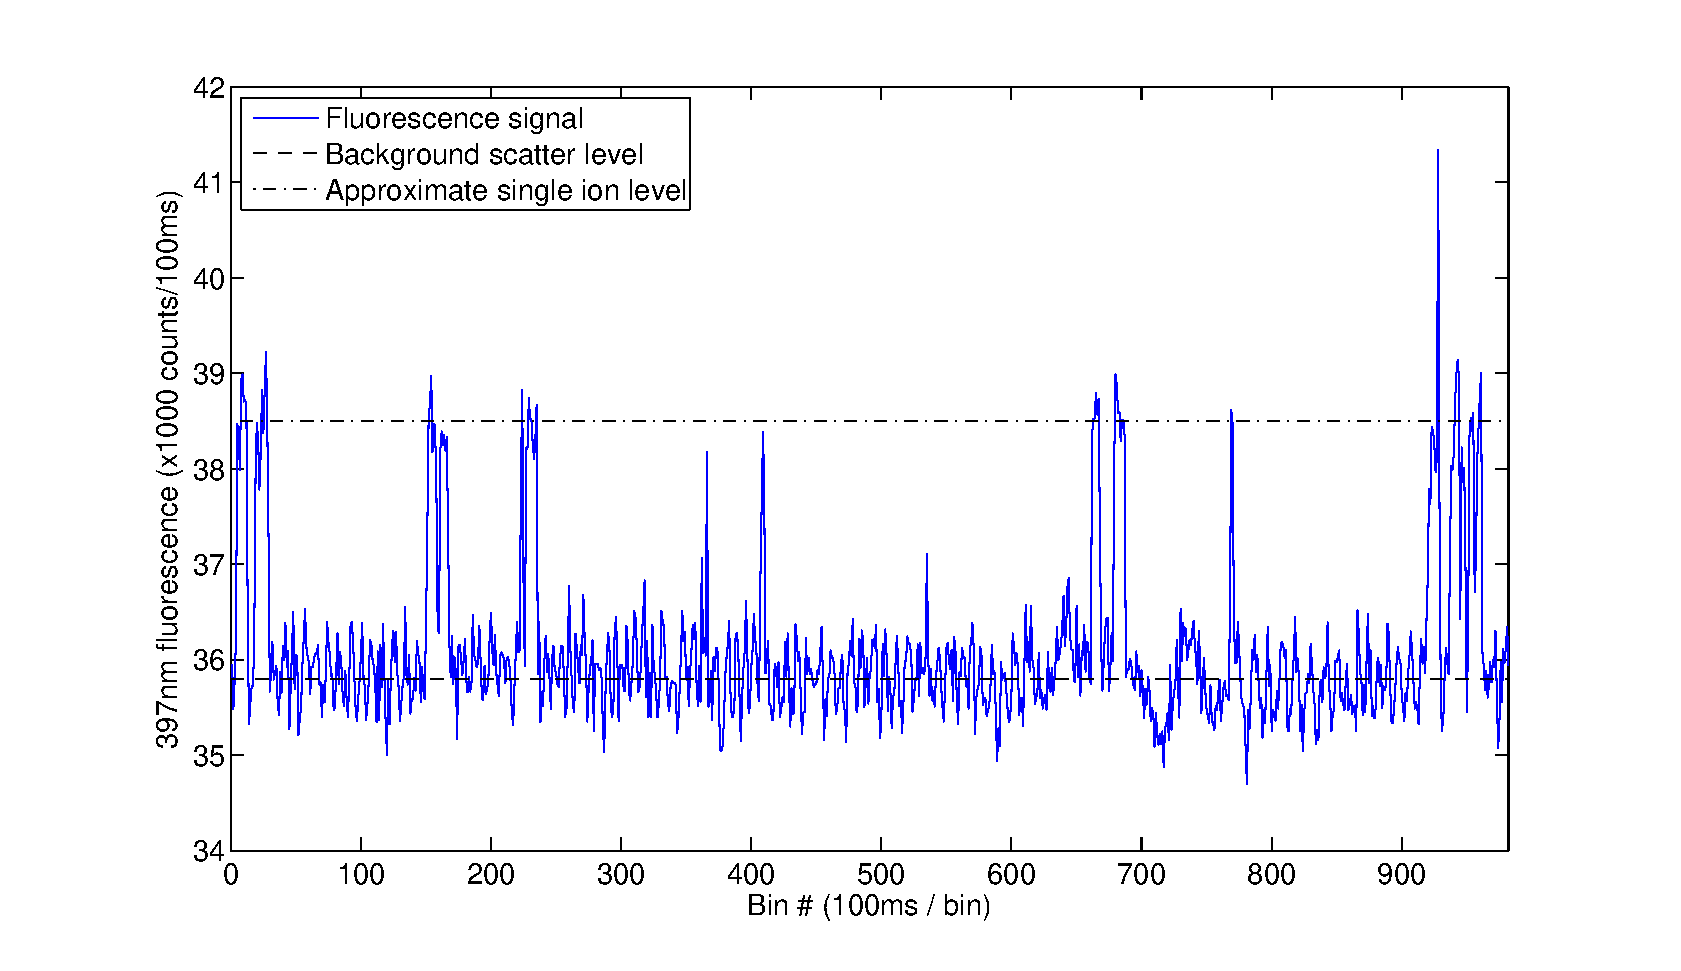
\includegraphics[width=14.5cm]{chapter6/firstion/firstionsign}
\caption[]{First proper single ion signal}
\label{firstionsign}
\end{figure} 



\begin{figure}[h!t]
\centering
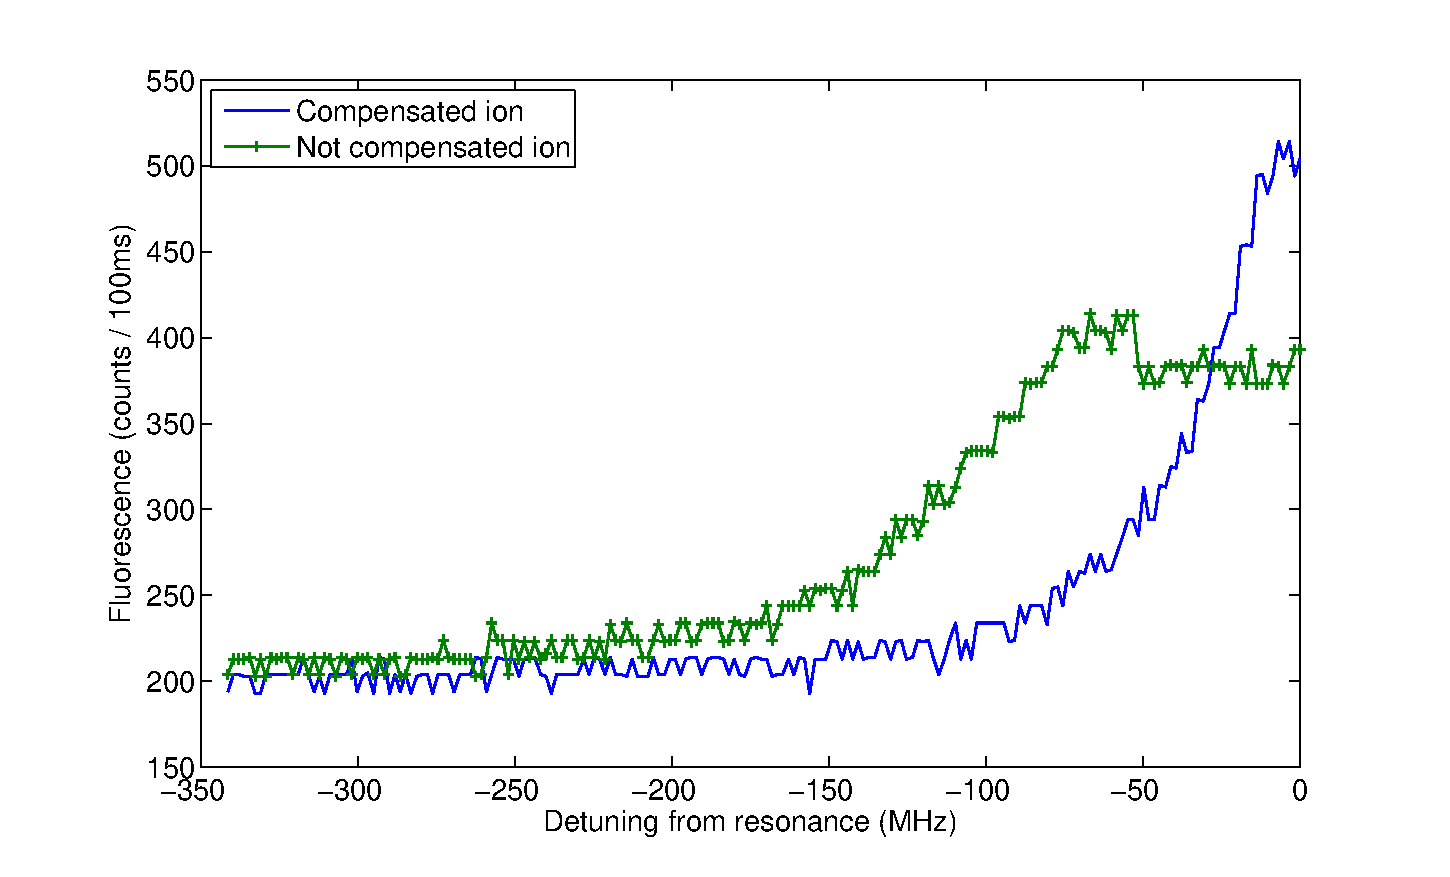
\includegraphics[width=14.5cm]{chapter6/rfcorr/compensation397_2}
\caption[]{397 scans showing Doppler-broadened and well compensated traces}
\label{397compensationscans}
\end{figure} 

\begin{figure}[h!t]
\centering
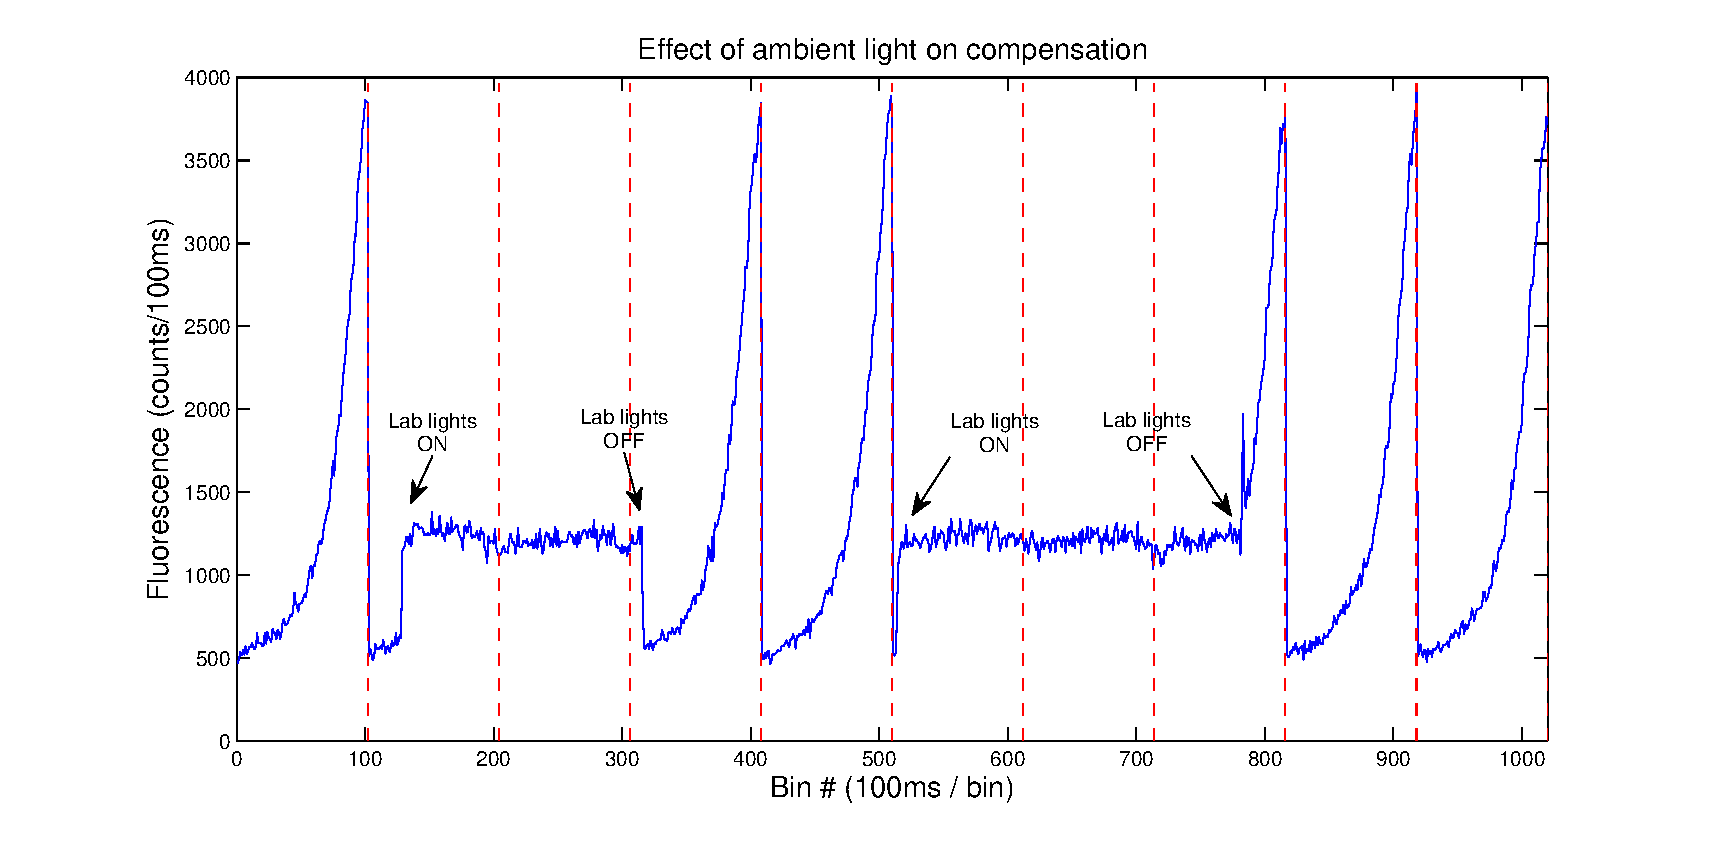
\includegraphics[width=14.5cm]{chapter6/lablights/lablights3}
\caption[Effect of ambient light on ion compensation]{Recorded fluorescence signal of repeated scans of the 397nm laser from red detuned to close to resonance with a range of approximately 132\MHz. The ion motion is compensated beforehand. The dashed vertical line separates the scans. The lab ambient lighting was turned on and off during the sequence, as it is shown on the plot. The signal during the those periods has a highly Doppler-broadened profile, and effectively flat in the scanned frequency region. }
\label{lablightingcompensate}
\end{figure} 

\begin{figure}[h!t]
\centering
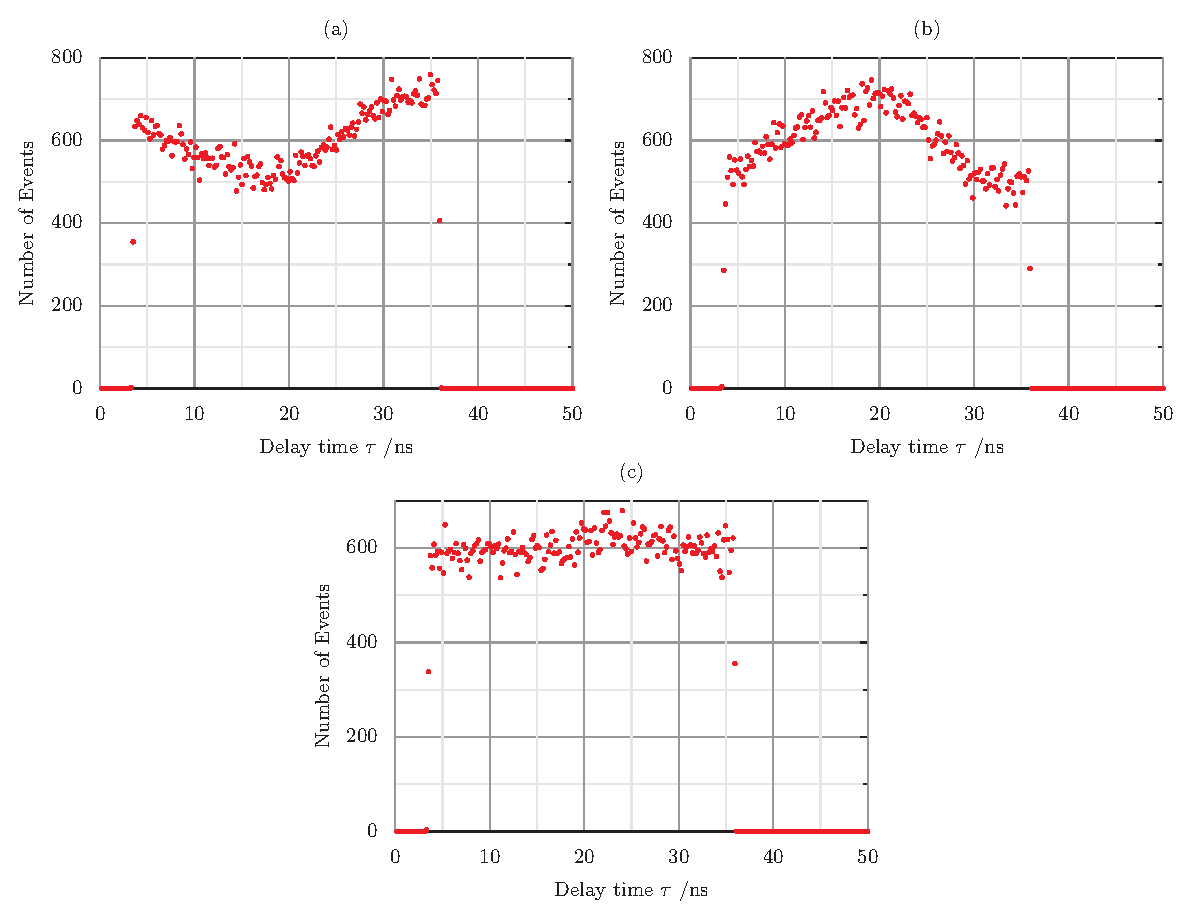
\includegraphics[width=14.5cm]{chapter6/rfcorr/rfexplots}
\caption[]{(a) under-compensated, (b) over-compensated, (c) well compensated. Plot from A. Myerson's first year report \cite{Myerson2007}.}
\label{rfcorrelation}
\end{figure} 



\begin{figure}[h!t]
\centering
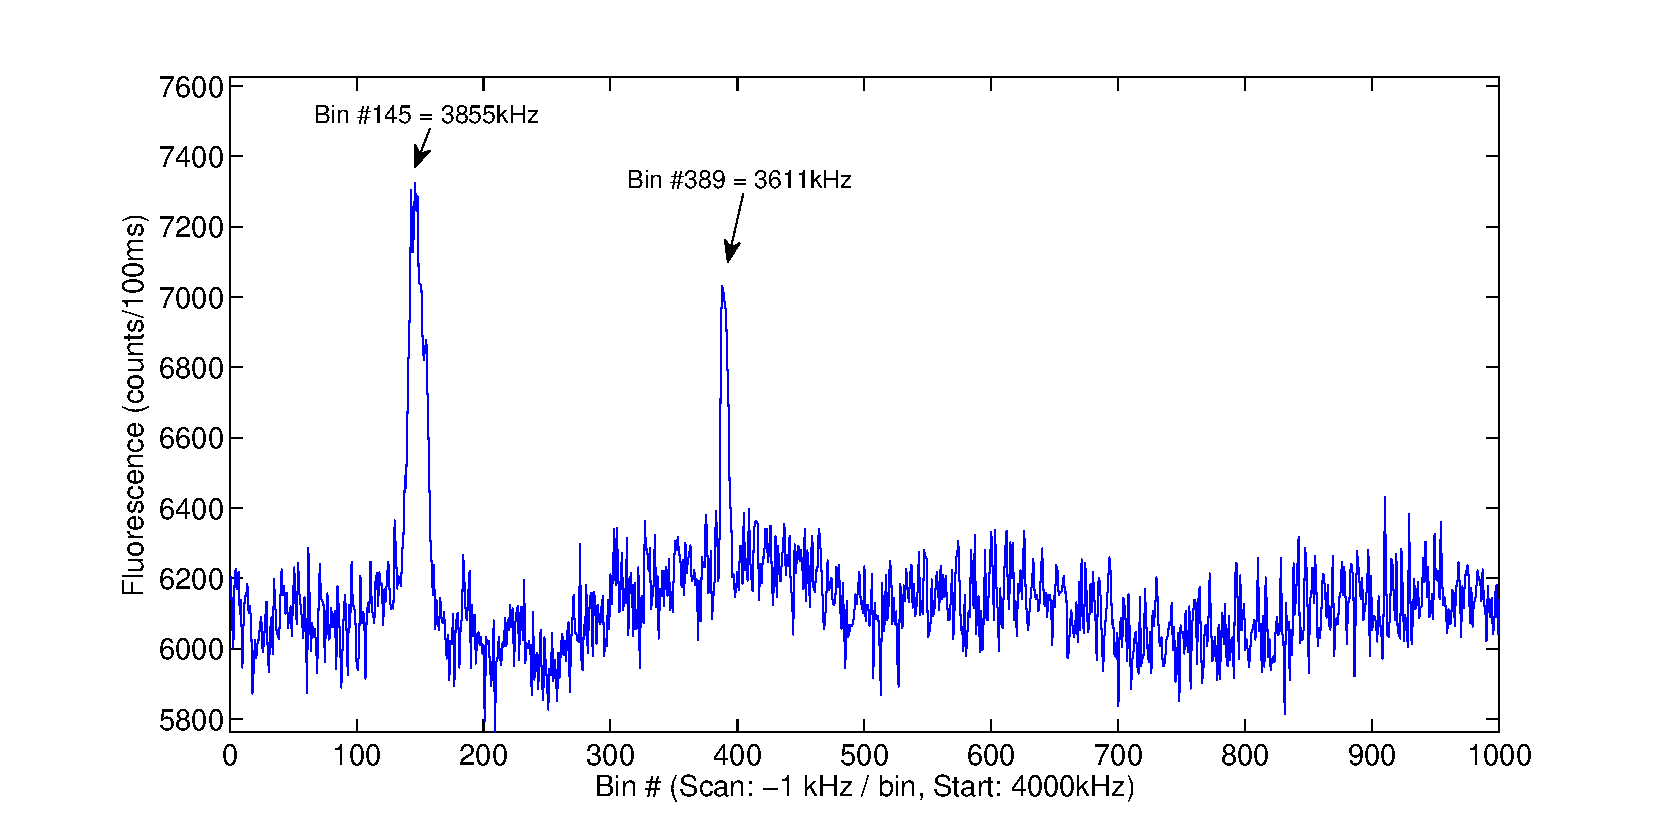
\includegraphics[width=14.5cm]{chapter6/tickle/ticklescan}
\caption[]{Scan of radial frequencies (with double peaks) precision ~$\pm 15 \kHz$.}
\label{ticklescan}
\end{figure} 

\begin{figure}[h!t]
\centering
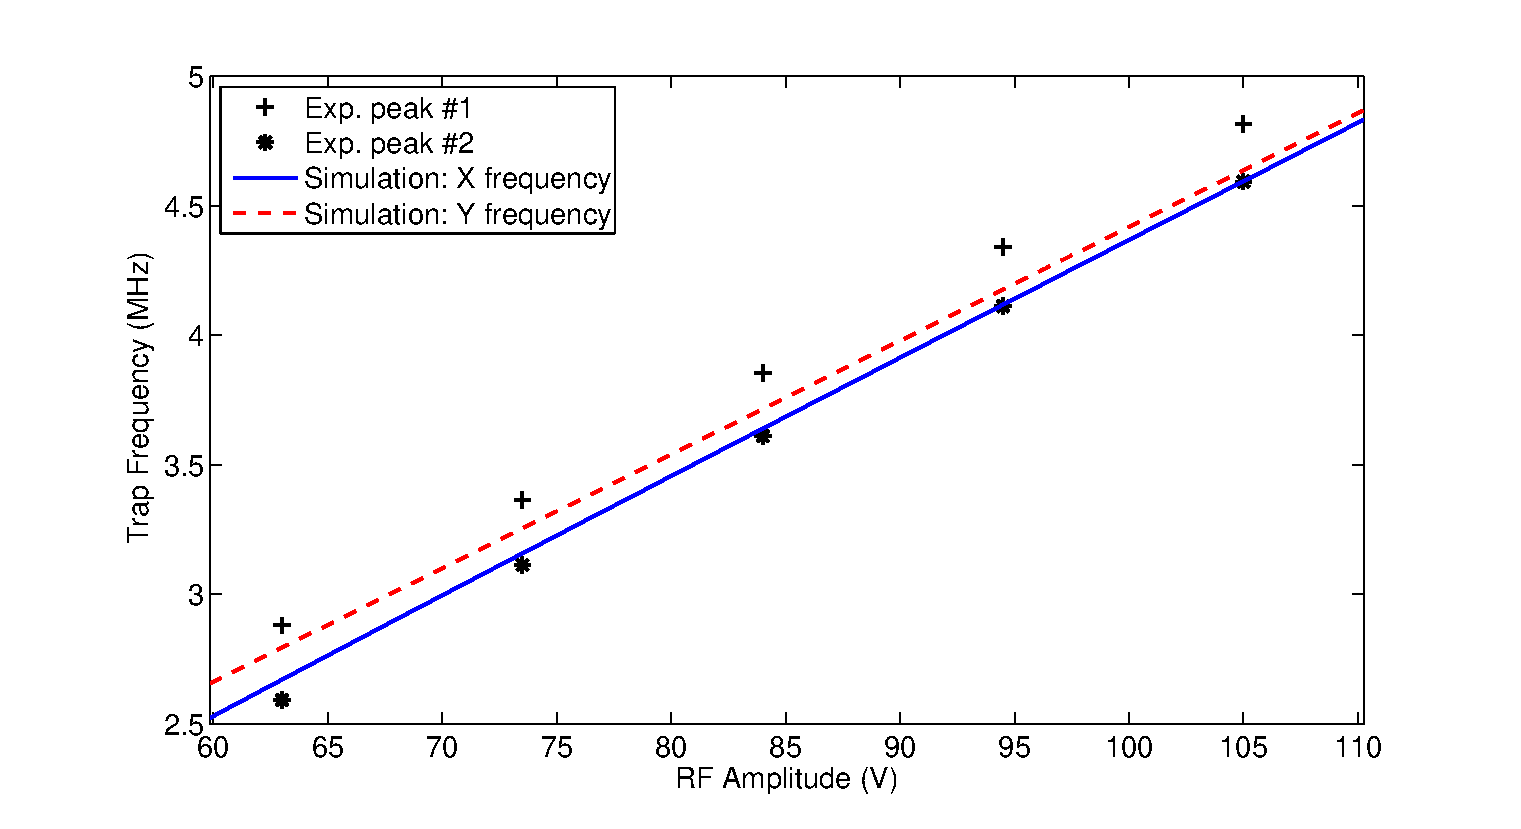
\includegraphics[width=14.5cm]{chapter6/tickle/radialtickle}
\caption[]{Radial frequencies - compared to simulation. Q value!}
\label{radialtickle}
\end{figure} 


\begin{figure}[h!t]
\centering
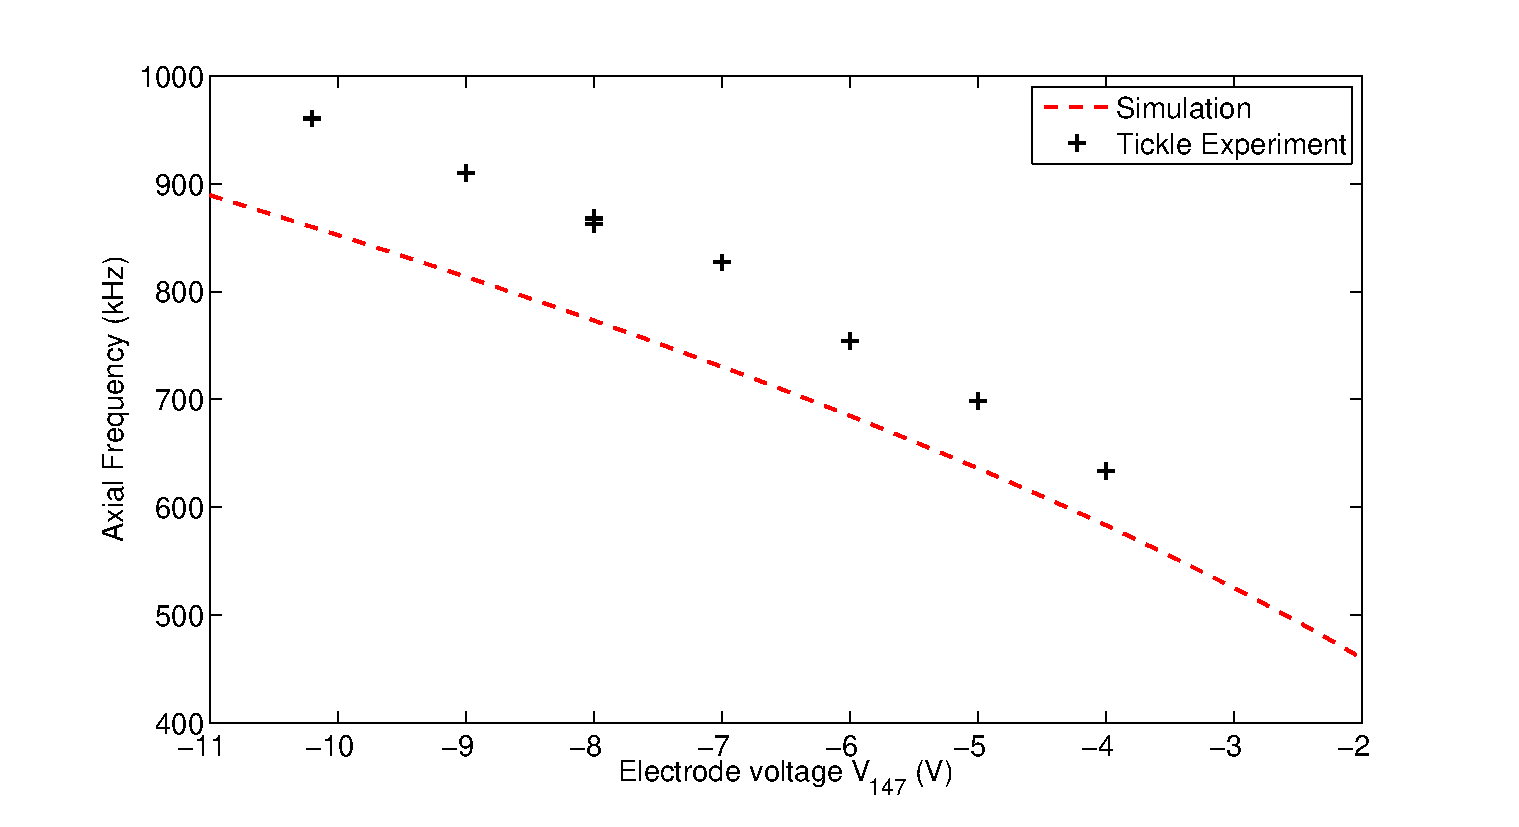
\includegraphics[width=14.5cm]{chapter6/tickle/axialtickle}
\caption[]{Recorded axial frequencies as a function of voltage - compared to simulation}
\label{axialtickle}
\end{figure} 



\begin{figure}[h!t]
\centering
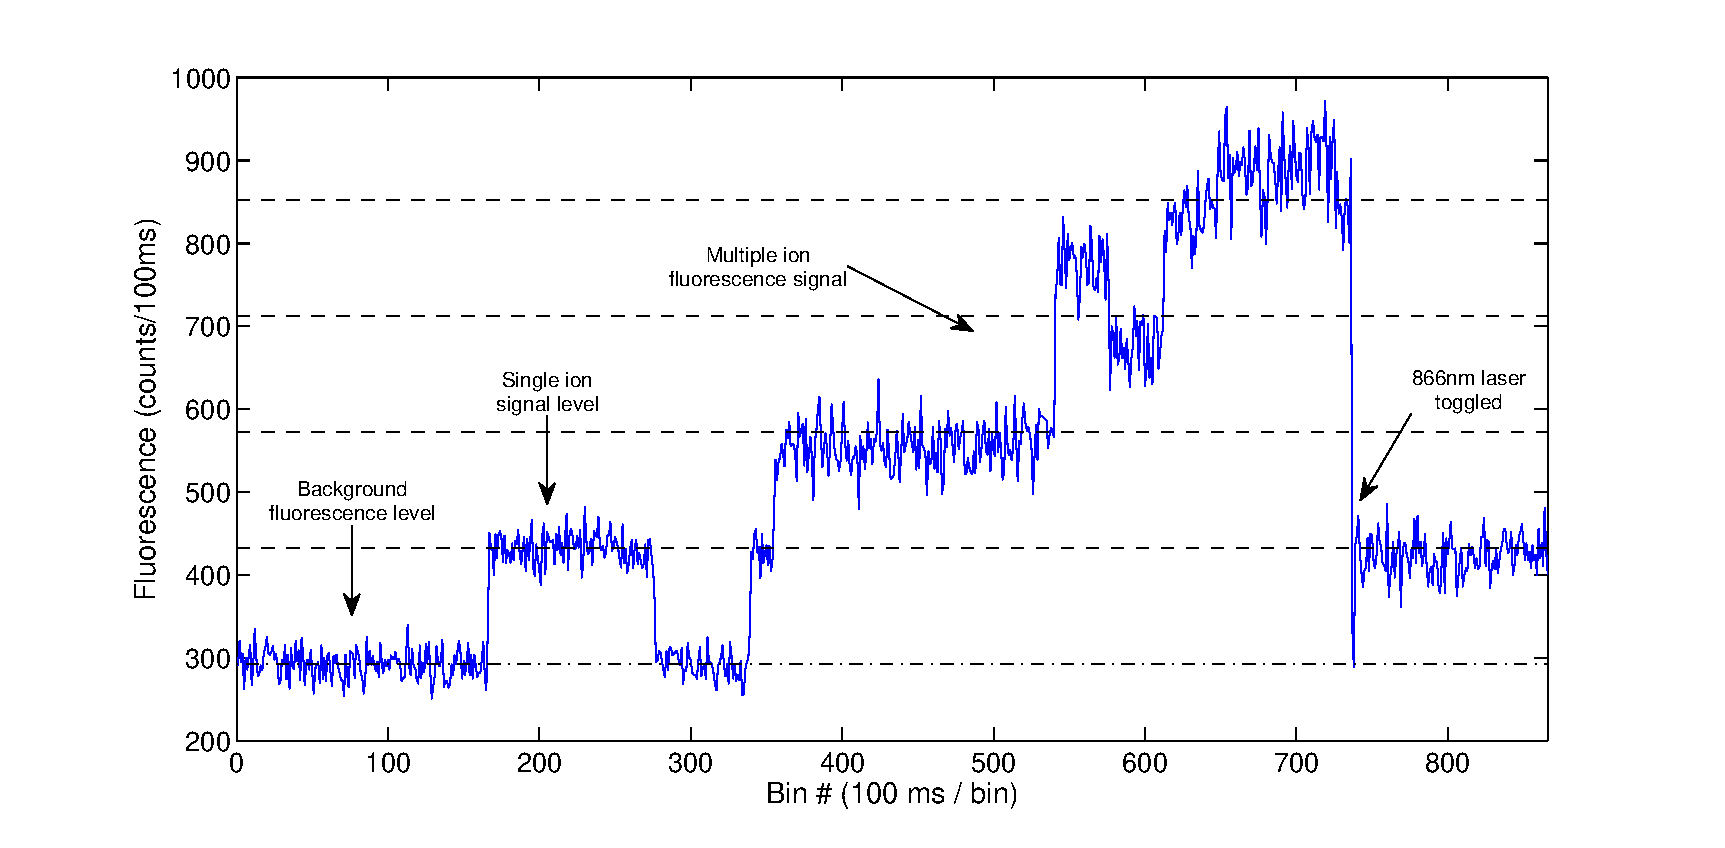
\includegraphics[width=14.5cm]{chapter6/multiload/multiload3}
\caption[Fluorescence signal of multiple loaded ions]{Fluorescence signal during ion loading. First a single ion is loaded. The \CaI{} oven, photoionization lasers and 854nm repumping laser were left on.  The signal shows a quantum jump like  behaviour, suggesting that multiple ions were trapped. Then the 866nm laser was toggled on/off quickly, which turns of the Doppler cooling of the ions for a short period of time. On the plot the \textit{dash-dotted} line represents the approximate background count level, while the \textit{dashed} lines show the approximate 1,2,3,4 ion signal levels, based on the single ion signal.}
\label{multiload}
\end{figure} 


\begin{figure}[h!t]
\centering
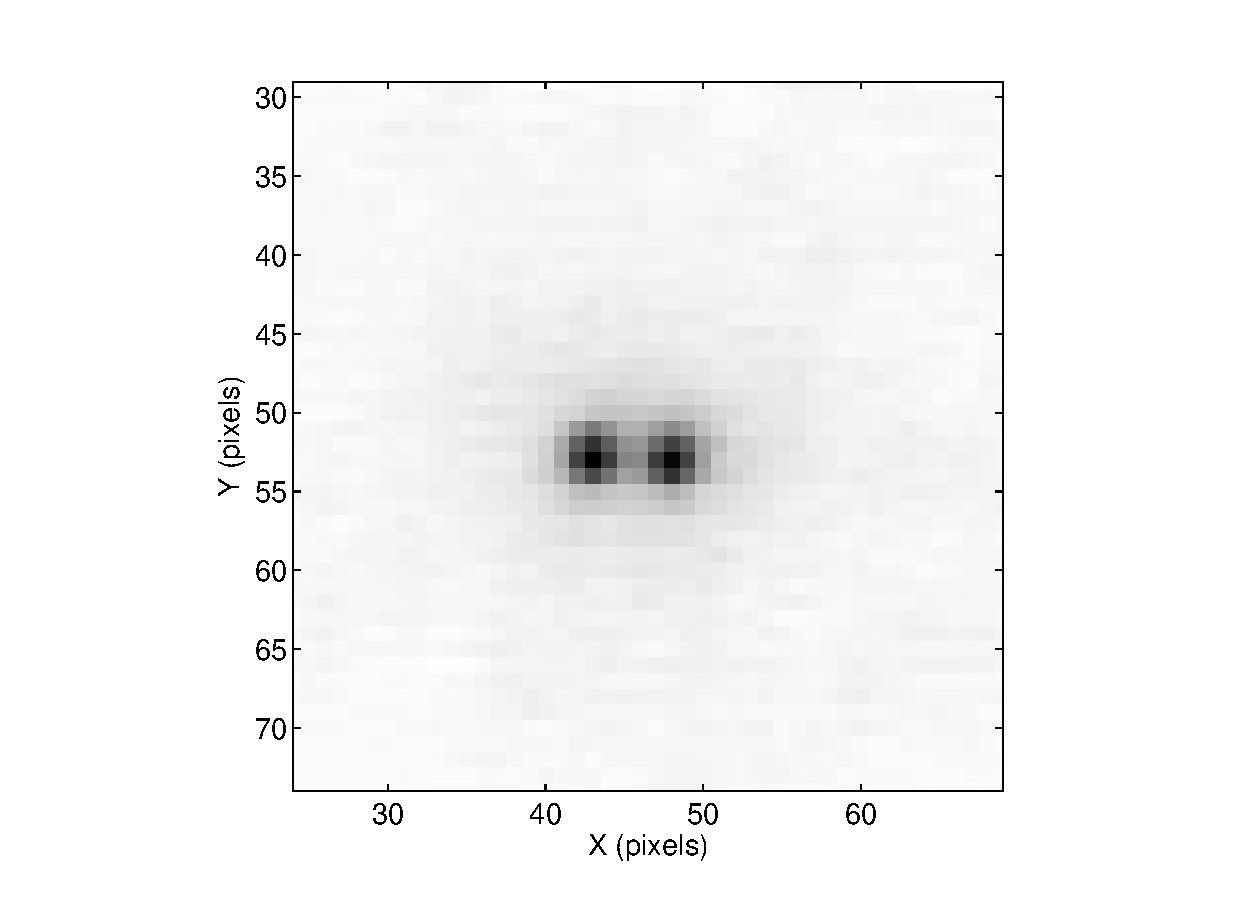
\includegraphics[width=11cm]{chapter6/twinion/twinionpic}
\caption[]{Pair of ions in the trap (maybe picture from gaussfit?) - Axial trap frequency ~ 317\kHz, Radial frequency ~ 2.7\MHz ($V_{RF} = 6Vpp$), scale: 15.3\um / pixel, 8x (??) magnification: separation = ? \um. }
\label{pairions}
\end{figure} 






